\chapter{Propuesta de solución}\label{chapter:proposal}

Este capítulo presenta una propuesta integral para abordar el desafío de la detección automática del cáncer de piel utilizando técnicas de aprendizaje profundo. La estrategia consiste en la utilización  de los pesos obtenidos de una red neuronal pre-entrenada y un algoritmo de ajuste de precisión, capaz de interpretar y clasificar imágenes dermatológicas. A continuación, se esbozan los enfoques metodológicos y las herramientas tecnológicas seleccionadas para llevar a cabo este proyecto.

\section{Desarrollo del modelo y estrategias de optimización}\label{sec:method}
%-----------------------------------------------------------------------------------

\subsection{Selección del modelo y transferencia de aprendizaje}

Como se explico anteriormente, el modelo consiste en utilizar los pesos obtenidos de una red neuronal convolucional pre-entrenada. Se optó por EfficientNetB1, una Red Neuronal Convolucional (CNN) pre-entrenada, como piedra angular del modelo. Esta elección se basa en la eficiencia de EfficientNet en términos de precisión y consumo de recursos computacionales \brackcite{tan2019efficientnet}. Al aprovechar un modelo pre-entrenado, se utilizan pesos obtenidos de extensos conjuntos de datos de imágenes, lo que facilita la adaptación a nuestro conjunto de datos específico. La omisión de la última capa de clasificación permite una personalización más profunda, adaptando el modelo para identificar con precisión las variadas presentaciones de tumores cutáneos presentes en el HAM1000.

\subsubsection{Arquitectura del modelo EfficientNet}
   
   La familia de arquitecturas EfficientNet, desarrollada por los autores en \brackcite{tan2019efficientnet}, surgió con el objetivo de hallar un método adecuado para escalar las CNNs de manera que mejoraran tanto en precisión (i.e., rendimiento del modelo) como en eficiencia (es decir, en términos de parámetros del modelo y FLOPS). Estos autores propusieron un método de escalado compuesto que utiliza un conjunto fijo de coeficientes para escalar de manera uniforme el ancho, la profundidad y la resolución de la red. El método les permitió desarrollar una arquitectura de CNN eficiente, a la que denominaron EfficientNet B0. Posteriormente, crearon las variantes EfficientNets B1-B7 escalando la red base (EfficientNet B0).
   
   Mientras que la arquitectura EfficientNet B0 tiene $5.3$ millones de parámetros y acepta imágenes de entrada de $224x224$, EfficientNet B7 cuenta con $66$ millones de parámetros y acepta imágenes de $600x600$ \brackcite{Tan2019EfficientNetRM}.
   
   \begin{figure}[ht]%
      \begin{center}
      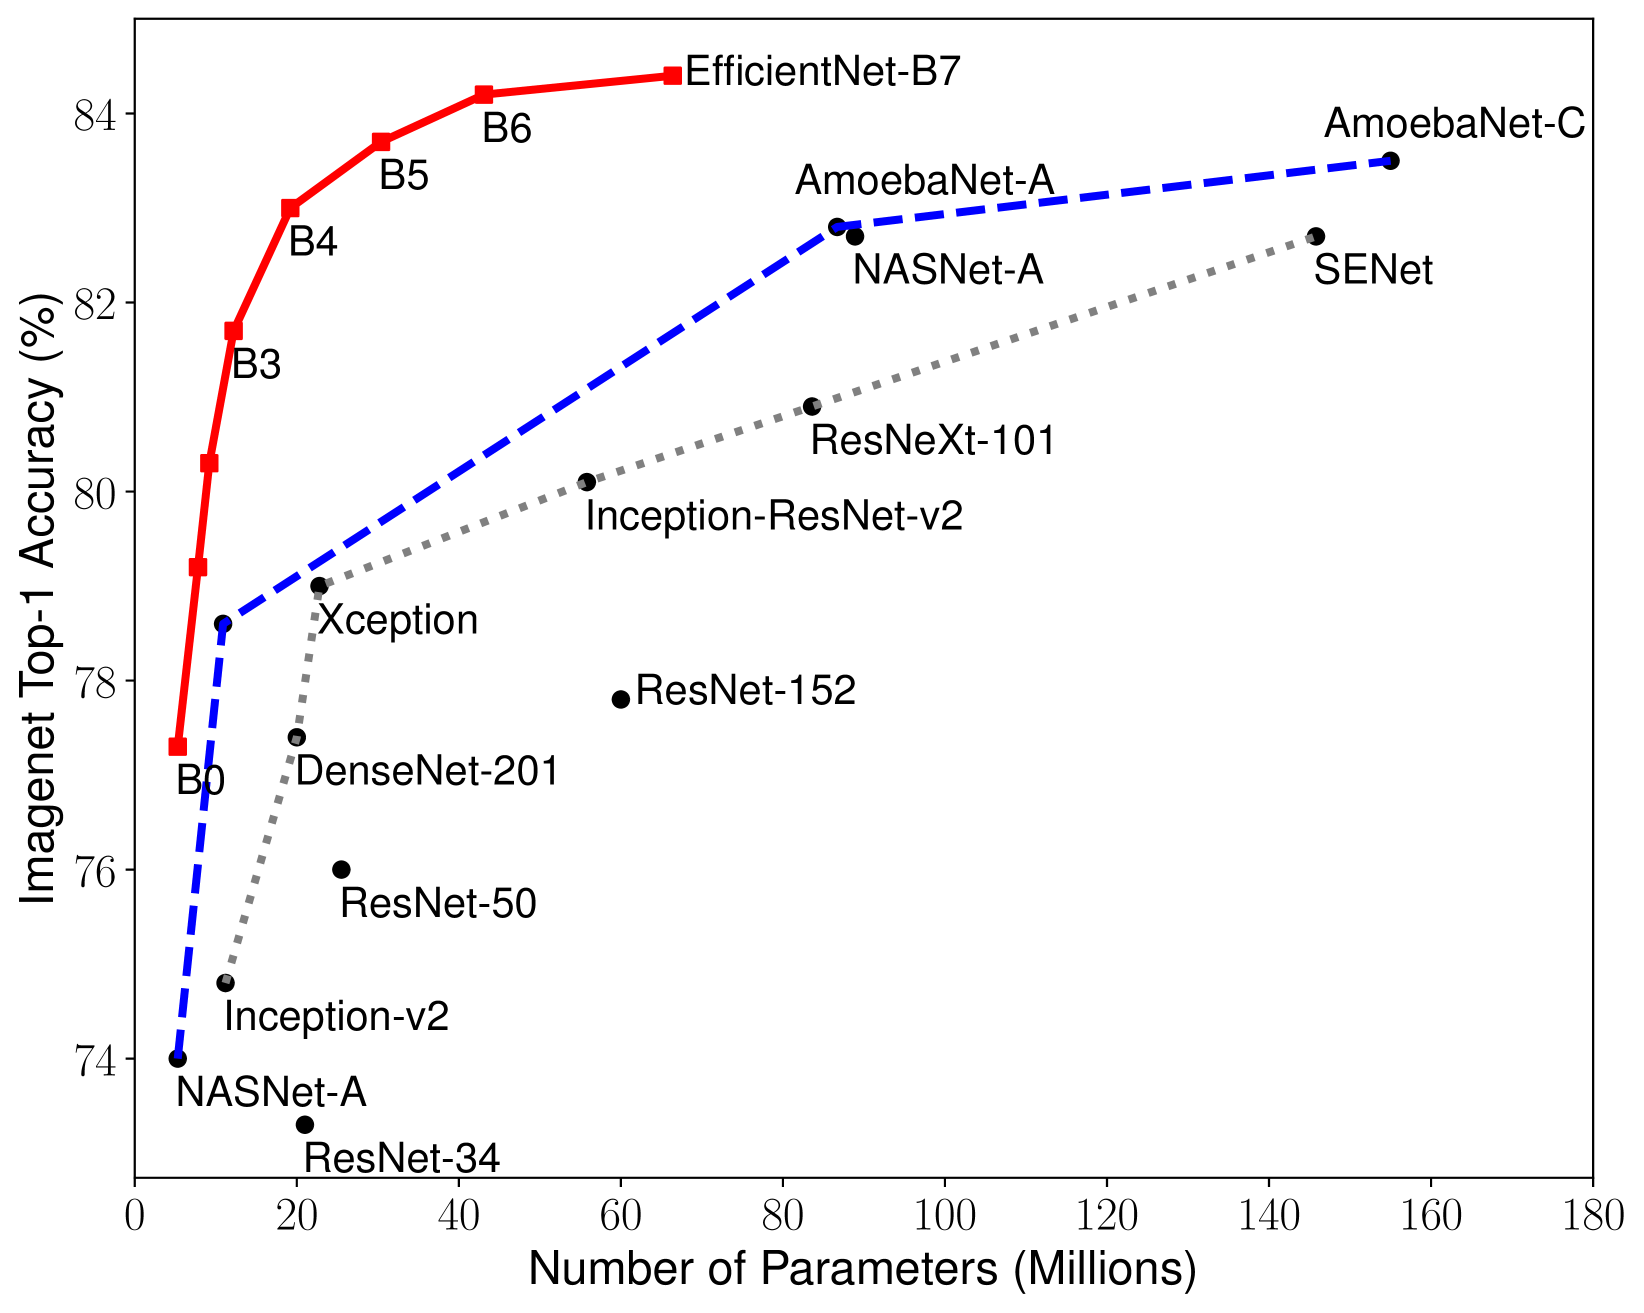
\includegraphics[width=1\textwidth]{./Graphics/efficientnet_performance.png}
      \caption{Estadísticas del rendimiento de los modelos de EfficientNet}
      \label{fig:efficientnet_performance}
      \end{center}
      \end{figure}
   
\subsubsection{EfficientNetB1}
   
   En relación con el dataset HAM1000 \brackcite{ham10000}, la implementación del EfficientNetB1 puede ser particularmente beneficiosa para el análisis de datos. EfficientNetB1, entre las variantes de la serie EfficientNet, se encuentra en un punto medio en términos de complejidad y tamaño, ofreciendo un equilibrio entre precisión y eficiencia computacional. Dado que el HAM1000 es un conjunto de datos de imágenes dermatoscópicas que requiere una alta precisión en la identificación y clasificación de lesiones cutáneas, la utilización de EfficientNetB5 podría proporcionar una precisión y eficiencia aceptable en términos de recursos computacionales.

\subsection{Preprocesamiento de datos y balanceo de clases}

El proceso de preprocesamiento incluye el re-dimensionamiento y la normalización de las imágenes, ajustándolas a los requisitos de entrada de EfficientNet. Dada la naturaleza del dataset HAM1000, que a menudo muestra un desequilibrio en la representación de clases, se puso especial énfasis en el balanceo de clases. Este paso es crucial para evitar sesgos en el modelo y asegurar que todas las categorías de tumores sean tratadas con igual importancia. Además, se empleó la técnica de aumento de datos para enriquecer el conjunto de entrenamiento, mejorando la capacidad del modelo para generalizar a partir de datos variados y no vistos anteriormente.

\subsection{Arquitectura del Modelo y Regularización}

Para fortalecer la arquitectura del modelo, se añadieron capas adicionales, incluyendo Dropout y regularizadores L1 y L2, esenciales para combatir el sobre-ajuste. Una capa densa personalizada fue incorporada para facilitar la clasificación precisa de múltiples tipos de tumores. La compilación del modelo se realizó con un enfoque en la clasificación multi-clase, utilizando la pérdida de entropía cruzada categórica y un optimizador adecuado, seleccionados por su efectividad en tareas similares.

\subsection{Ajuste dinámico del learning rate}

Un elemento innovador del entrenamiento fue la implementación de un callback personalizado para el ajuste dinámico del learning rate. Esta estrategia permite ajustes adaptativos del learning rate basados en el rendimiento del modelo, optimizando la eficiencia del entrenamiento y evitando el estancamiento en mínimos locales del espacio de búsqueda.

\subsection{Diversidad en propuestas de soluciones}

El proyecto explora diferentes enfoques tanto en el preprocesamiento de datos como en la elección de optimizadores. Esta variedad en las técnicas utilizadas refleja un esfuerzo por abordar el problema desde múltiples perspectivas, aumentando así las probabilidades de encontrar la solución más eficaz para el desafío específico del dataset HAM1000.